% Autor: Elias Welt
\section{KI-Chat (Chat.jsx)}

Die Chat-Komponente bietet eine Schnittstelle zu einem Large Language Model (LLM) und ist damit das KI-Herzstück von EduShelf. Sie erlaubt es, Lernmaterial direkt mit einem KI-Assistenten zu besprechen, Fragen zu stellen und Bilder als Kontext mitzuschicken.

\begin{figure}[h]
    \centering
    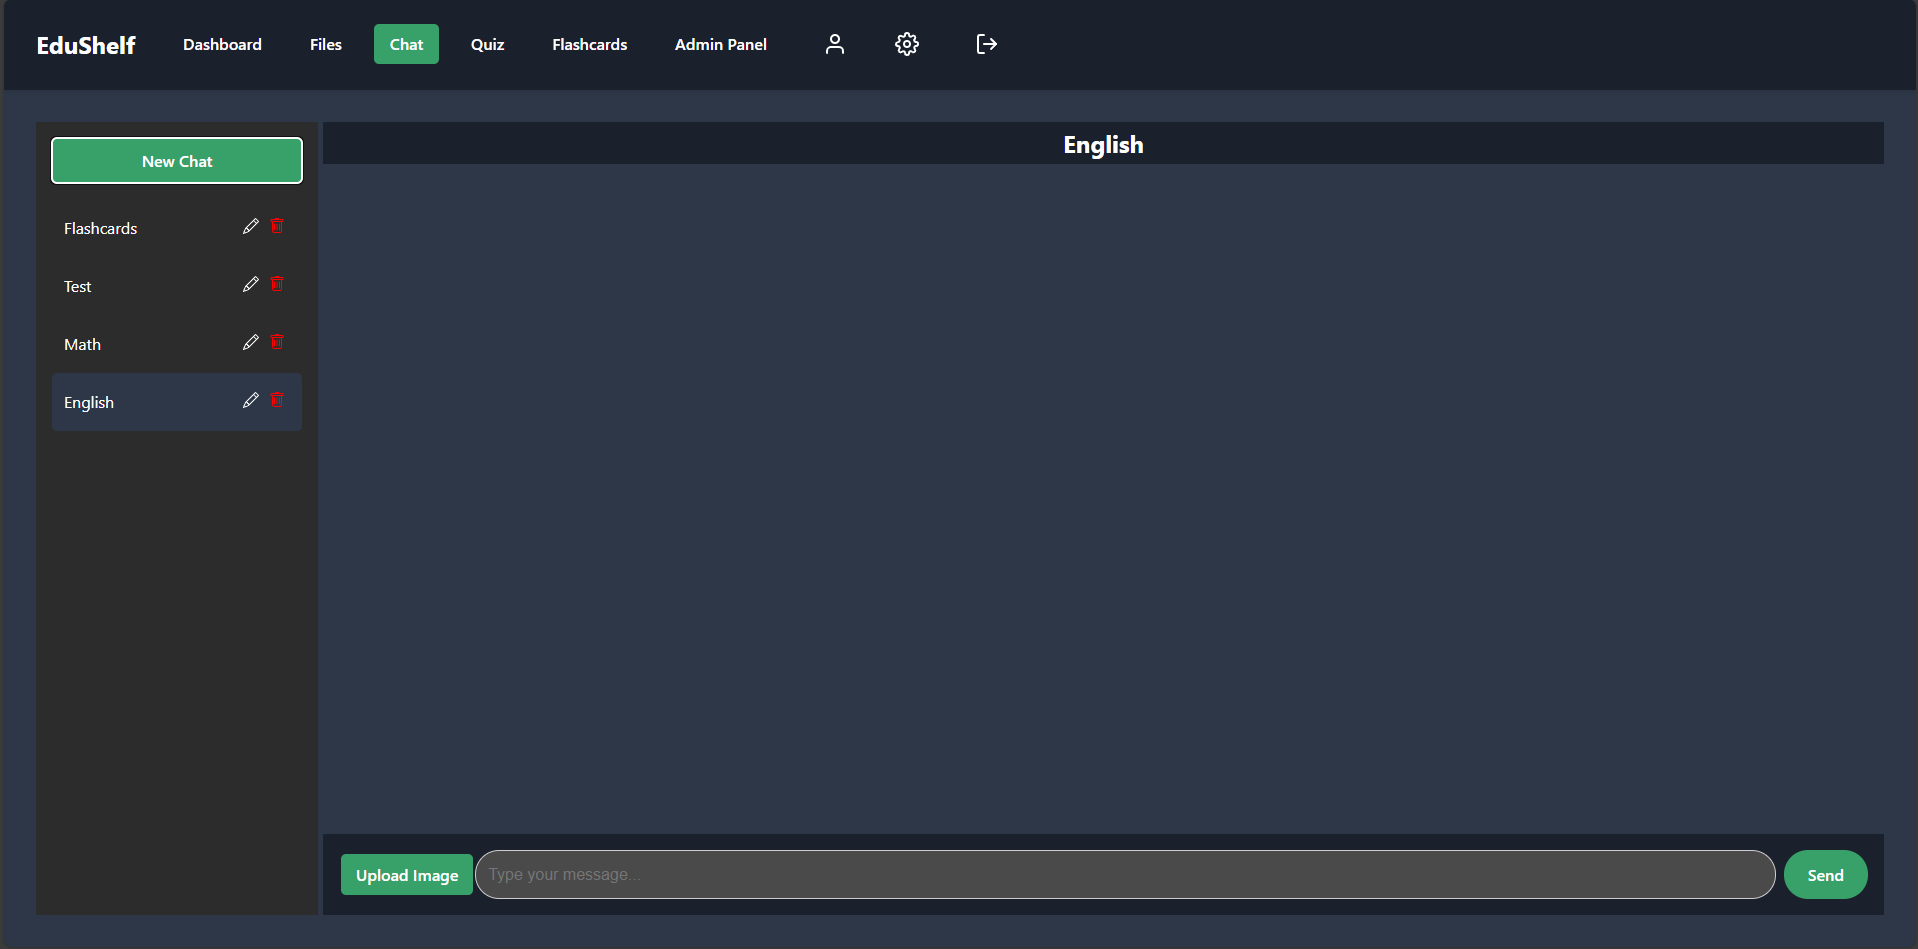
\includegraphics[width=0.92\textwidth]{img/chat-dark-mode}
    \caption{KI-Chat-Ansicht von EduShelf im Dark-Mode}
    \label{fig:chat}
\end{figure}


\subsection{Implementierungsdetails}

\subsubsection{Request/Response-Pattern}

Die aktuelle Implementierung wartet auf die vollständige Antwort des Servers (Request/Response Pattern). Während des Wartens wird ein \textit{Thinking Indicator} -- drei animierte Punkte -- über den \texttt{isLoading}-State eingeblendet. Der Eingabebereich wird in dieser Zeit deaktiviert, um doppelte Anfragen zu verhindern.
\newpage

\subsubsection{Markdown-Rendering}

Da KI-Modelle häufig strukturierten Text mit Codeblöcken und Listen ausgeben, wird \texttt{react-markdown} in Kombination mit \texttt{rehype-highlight} verwendet. Diese Bibliotheken konvertieren die Markdown-Antwort sicher in HTML und bieten Syntax-Highlighting für Codeblöcke:

\begin{lstlisting}[language=JavaScript, caption={Markdown-Rendering mit Syntax-Highlighting}]
import ReactMarkdown from 'react-markdown';
import rehypeHighlight from 'rehype-highlight';

<ReactMarkdown rehypePlugins={[rehypeHighlight]}>
    {message.content}
</ReactMarkdown>
\end{lstlisting}

\subsubsection{Bildupload als Input}

Benutzer können Bilder als Kontext an das Modell übermitteln. Das gewählte Bild wird mittels \texttt{URL.createObjectURL()} sofort lokal in einer Vorschau angezeigt, bevor es als Blob an den Server gesendet wird. Dies gibt dem Nutzer unmittelbares visuelles Feedback, ohne auf die Serverantwort warten zu müssen.

\begin{figure}[h]
    \centering
    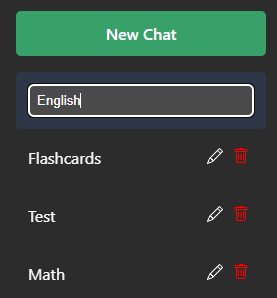
\includegraphics[width=0.35\textwidth]{img/edit-chat-dark-mode}
    \caption{Chat-Eingabebereich mit Bildupload-Option}
    \label{fig:chat-edit}
\end{figure}

